%\documentclass[a4paper]{hitec}
\documentclass[a4paper,UKenglish,cleveref, autoref]{lipics-v2019}

%%% PGF Plots
\usepackage{pgfplots}
\pgfplotsset{width=5cm,compat=1.16}
\usepgfplotslibrary{statistics,groupplots}
\usetikzlibrary{patterns}
%\usetikzlibrary{external}
%\tikzexternalize[prefix=./tikzcache/]
%\tikzexternalenable
\usepackage{pgfplotstable}

\newenvironment{customlegend}[1][]{%
    \begingroup
    % inits/clears the lists (which might be populated from previous
    % axes):
    \csname pgfplots@init@cleared@structures\endcsname
    \pgfplotsset{#1}%
}{%
    % draws the legend:
    \csname pgfplots@createlegend\endcsname
    \endgroup
}%

% makes \addlegendimage available (typically only available within an
% axis environment):
\def\addlegendimage{\csname pgfplots@addlegendimage\endcsname}


%%%%%%%%%%%%%%%%%%%%%%%%%%%%%%%%%%%%%%%%%%%%%%%%%%%%%%%%%%%%%%%%%%%%%%%%%%%%%%%%
\title{Artifact evaluation for Novel methodologies for predictable CPU-to-GPU command offloading}

\author{Roberto Cavicchioli}{University of Modena and Reggio Emilia, Italy}{roberto.cavicchioli@unimore.it}{}{}
\author{Nicola Capodieci}{University of Modena and Reggio Emilia, Italy}{nicola.capodieci@unimore.it}{}{}
\author{Marco Solieri}{University of Modena and Reggio Emilia, Italy}{marco.solieri@unimore.it}{}{}
\author{Marko Bertogna}{University of Modena and Reggio Emilia, Italy}{marko.bertogna@unimore.it}{}{}
%%%%%%%%%%%%%%%%%%%%%%%%%%%%%%%%%%%%%%%%%%%%%%%%%%%%%%%%%%%%%%%%%%%%%%%%%%%%%%%%
\begin{document}

\maketitle


\pgfplotscreateplotcyclelist{exotic}{
  teal,every mark/.append style={fill=teal!80!black},mark=*\\
  orange,every mark/.append style={fill=orange!80!black},mark=square*\\
  cyan!60!black,every mark/.append style={fill=cyan!80!black},mark=diamond*\\
  red!70!white,mark=star\\
}
\pgfplotscreateplotcyclelist{exotic2}{
  lime!80!black,every mark/.append style={fill=lime},mark=diamond*\\
  red,densely dashed,every mark/.append style={solid,fill=red!80!black},mark=*\\
}

\pagebreak
\centering

%%%%%%%%%%%%%%%%%%%%%%%%%%%%%%%%%%%%%%%%%%%%%%%%%%%%%%%%%%%%%%%%%%%%
% NEW DATA, NEW FORMAT
%%%%%%%%%%%%%%%%%%%%%%%%%%%%%%%%%%%%%%%%%%%%%%%%%%%%%%%%%%%%%%%%%%%%
%%% l \in {1,2,5,10,20,50}
\begin{tikzpicture}
  \begin{groupplot}[
      group style={
        group size=2 by 4,
        xlabels at=edge bottom,
        horizontal sep=1cm,
        vertical sep=0.25cm,
      },
      boxplot/draw direction=y,
      footnotesize,
      width=.6\textwidth,
      height=.3\textheight,
      ymode=log,
      cycle list name=exotic,
      xtick={0.5,4.5,8.5,12.5,16.5,20.5,24.5},
      xticklabels={},
      xticklabel style={anchor=north west},
      xlabel style={align=center},
      ylabel style={align=center},
      xmajorgrids,
      ymajorgrids,
    ]
    %%% Size = 1
    \nextgroupplot[
      ylabel={$ k=1 $\\Response time $\left[ s \right]$},
    ]
    \pgfplotsforeachungrouped \tasksize in {1,2,5,10,20,50} {
      \pgfplotsforeachungrouped \submission in {baseline,CNP,graph,vulkan} {
        \addplot+ [boxplot] table [y expr=\thisrow{\submission:sub:i\tasksize:s1}]
           {results_artifact.csv};
      }
    }
    \nextgroupplot
    \pgfplotsforeachungrouped \tasksize in {1,2,5,10,20,50} {
      \pgfplotsforeachungrouped \submission in {baseline,CNP,graph,vulkan} {
        \addplot+ [boxplot] table [y expr=\thisrow{\submission:exe:i\tasksize:s1}]
           {results_artifact.csv};
      }
    }
    %%% Size = 2
    \nextgroupplot[
      ylabel={$ k=2 $\\Response time $\left[ s \right]$},
    ]
    \pgfplotsforeachungrouped \tasksize in {1,2,5,10,20,50} {
      \pgfplotsforeachungrouped \submission in {baseline,CNP,graph,vulkan} {
        \addplot+ [boxplot] table [y expr=\thisrow{\submission:sub:i\tasksize:s2}]
           {results_artifact.csv};
      }
    }
    \nextgroupplot
    \pgfplotsforeachungrouped \tasksize in {1,2,5,10,20,50} {
      \pgfplotsforeachungrouped \submission in {baseline,CNP,graph,vulkan} {
        \addplot+ [boxplot] table [y expr=\thisrow{\submission:exe:i\tasksize:s2}]
           {results_artifact.csv};
      }
    }
    %%% Size = 4
    \nextgroupplot[
      ylabel={$ k=4 $\\Response time $\left[ s \right]$},
    ]
    \pgfplotsforeachungrouped \tasksize in {1,2,5,10,20,50} {
      \pgfplotsforeachungrouped \submission in {baseline,CNP,graph,vulkan} {
        \addplot+ [boxplot] table [y expr=\thisrow{\submission:sub:i\tasksize:s4}]
           {results_artifact.csv};
      }
    }
    \nextgroupplot
    \pgfplotsforeachungrouped \tasksize in {1,2,5,10,20,50} {
      \pgfplotsforeachungrouped \submission in {baseline,CNP,graph,vulkan} {
        \addplot+ [boxplot] table [y expr=\thisrow{\submission:exe:i\tasksize:s4}]
           {results_artifact.csv};
      }
    }
    %%% Size = 8
    \nextgroupplot[
      xticklabels={1,5,10,50,100,500},
      xlabel={Submission length $ l $\\\emph{Submission}},
      ylabel={$ k=8 $\\Response time $\left[ s \right]$},
    ]
    \pgfplotsforeachungrouped \tasksize in {1,2,5,10,20,50} {
      \pgfplotsforeachungrouped \submission in {baseline,CNP,graph,vulkan} {
        \addplot+ [boxplot] table [y expr=\thisrow{\submission:sub:i\tasksize:s8}]
           {results_artifact.csv};
      }
    }
    \nextgroupplot[
      xticklabels={1,5,10,50,100,500},
      xlabel={Submission length $ l $}\\\emph{Execution},
    ]
    \pgfplotsforeachungrouped \tasksize in {1,2,5,10,20,50} {
      \pgfplotsforeachungrouped \submission in {baseline,CNP,graph,vulkan} {
        \addplot+ [boxplot] table [y expr=\thisrow{\submission:exe:i\tasksize:s8}]
           {results_artifact.csv};
      }
    }
  \end{groupplot}
\end{tikzpicture}

%%%%%%%%%%%%%%%%%%%%%%%%%%%%%%%%%%%%%%%%%%%%%%%%%%%%%%%%%%%%%%%%%%%%
%%% l \in {100,200,500,1000,2000}
%%%%%%%%%%%%%%%%%%%%%%%%%%%%%%%%%%%%%%%%%%%%%%%%%%%%%%%%%%%%%%%%%%%%
\begin{tikzpicture}
  \begin{groupplot}[
      group style={
        group size=2 by 4,
        xlabels at=edge bottom,
        horizontal sep=1cm,
        vertical sep=0.25cm,
      },
      boxplot/draw direction=y,
      footnotesize,
      width=.6\textwidth,
      height=.3\textheight,
      ymode=log,
      cycle list name=exotic,
      xtick={0.5,4.5,8.5,12.5,16.5,20.5,24.5},
      xticklabels={},
      xticklabel style={anchor=north west},
      xlabel style={align=center},
      ylabel style={align=center},
      xmajorgrids,
      ymajorgrids,
    ]
    %%% Size = 1
    \nextgroupplot[
      ylabel={$ k=1 $\\Response time $\left[ s \right]$},
    ]
    \pgfplotsforeachungrouped \tasksize in {100,200,500,1000,2000} {
      \pgfplotsforeachungrouped \submission in {baseline,CNP,graph,vulkan} {
        \addplot+ [boxplot] table [y expr=\thisrow{\submission:sub:i\tasksize:s1}]
           {results_artifact.csv};
      }
    }
    \nextgroupplot
    \pgfplotsforeachungrouped \tasksize in {100,200,500,1000,2000} {
      \pgfplotsforeachungrouped \submission in {baseline,CNP,graph,vulkan} {
        \addplot+ [boxplot] table [y expr=\thisrow{\submission:exe:i\tasksize:s1}]
           {results_artifact.csv};
      }
    }
    %%% Size = 2
    \nextgroupplot[
      ylabel={$ k=2 $\\Response time $\left[ s \right]$},
    ]
    \pgfplotsforeachungrouped \tasksize in {100,200,500,1000,2000} {
      \pgfplotsforeachungrouped \submission in {baseline,CNP,graph,vulkan} {
        \addplot+ [boxplot] table [y expr=\thisrow{\submission:sub:i\tasksize:s2}]
           {results_artifact.csv};
      }
    }
    \nextgroupplot
    \pgfplotsforeachungrouped \tasksize in {100,200,500,1000,2000} {
      \pgfplotsforeachungrouped \submission in {baseline,CNP,graph,vulkan} {
        \addplot+ [boxplot] table [y expr=\thisrow{\submission:exe:i\tasksize:s2}]
           {results_artifact.csv};
      }
    }
    %%% Size = 4
    \nextgroupplot[
      ylabel={$ k=4 $\\Response time $\left[ s \right]$},
    ]
    \pgfplotsforeachungrouped \tasksize in {100,200,500,1000,2000} {
      \pgfplotsforeachungrouped \submission in {baseline,CNP,graph,vulkan} {
        \addplot+ [boxplot] table [y expr=\thisrow{\submission:sub:i\tasksize:s4}]
           {results_artifact.csv};
      }
    }
    \nextgroupplot
    \pgfplotsforeachungrouped \tasksize in {100,200,500,1000,2000} {
      \pgfplotsforeachungrouped \submission in {baseline,CNP,graph,vulkan} {
        \addplot+ [boxplot] table [y expr=\thisrow{\submission:exe:i\tasksize:s4}]
           {results_artifact.csv};
      }
    }
    %%% Size = 8
    \nextgroupplot[
      xticklabels={100,200,500,1000,2000},
      xlabel={Submission length $ l $\\\emph{Submission}},
      ylabel={$ k=8 $\\Response time $\left[ s \right]$},
      name=reflegend,
    ]
    \pgfplotsforeachungrouped \tasksize in {100,200,500,1000,2000} {
      \pgfplotsforeachungrouped \submission in {baseline,CNP,graph,vulkan} {
        \addplot+ [boxplot] table [y expr=\thisrow{\submission:sub:i\tasksize:s8}]
           {results_artifact.csv};
      }
    }
    \nextgroupplot[
      xticklabels={100,200,500,1000,2000},
      xlabel={Submission length $ l $}\\\emph{Execution},
    ]
    \pgfplotsforeachungrouped \tasksize in {100,200,500,1000,2000} {
      \pgfplotsforeachungrouped \submission in {baseline,CNP,graph,vulkan} {
        \addplot+ [boxplot] table [y expr=\thisrow{\submission:exe:i\tasksize:s8}]
           {results_artifact.csv};
      }
    }
  \end{groupplot}
\end{tikzpicture}

%%%%%%%%%%%%%%%%%%%%%%%%%%%%%%%%%%%%%%%%%%%%%%%%%%%%%%%%%%%%%%%%%%%%
% legend-generating dummy plot
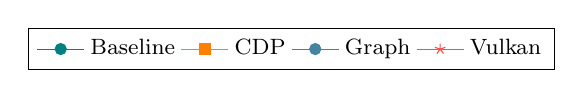
\begin{tikzpicture}
    \begin{axis}[
      hide axis,
      footnotesize,
      legend style={
        at={(1,0.55)},
        anchor=north,
        legend columns=-1,
      },
      cycle list name=exotic,
      legend entries = {Baseline, CDP, Graph, Vulkan},
    ],
    \addplot {0};\addplot {0};\addplot {0};\addplot {0};
  \end{axis}
\end{tikzpicture}
\clearpage
%%%%%%%%%%%%%%%%%%%%%%%%%%%%%%%%%%%%%%%%%%%%%%%%%%%%%%%%%%%%%%%%%%%%
% Jitter
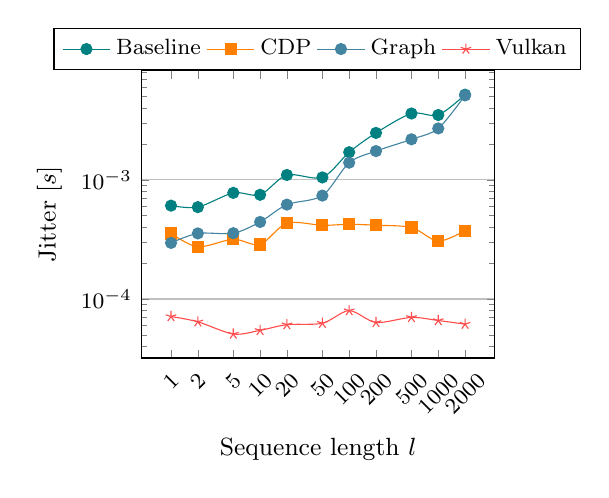
\begin{tikzpicture}
  \centering
  \begin{axis}[
    footnotesize,
    width=0.5\textwidth,
    smooth,
    xtick={1,2,5,10,20,50,100,200,500,1000,2000},
    xticklabels={1,2,5,10,20,50,100,200,500,1000,2000},
    xticklabel style={rotate=45},
    xmode=log,
    ymode=log,
    xlabel={Sequence length $l$},
    ylabel={Jitter $\left[ s \right]$},
    ymajorgrids,
    legend style={
      at={(-0.25,1.15)},
      anchor=north west,
      cells={anchor=west},
      legend columns=4,
      },
    cycle list name=exotic,
    ]
\addplot+ [] table {
1               0.000607128
2               0.0005898480000000001
5               0.000776991
10              0.0007484760000000001
20              0.00109736
50              0.0010467599999999999
100             0.0017029099999999998
200             0.00247206
500             0.003597699999999997
1000            0.0034944000000000017
2000            0.005173299999999999
};
%CNP:sub
\addplot+ [] table {
1               0.00035499
2               0.00027402700000000004
5               0.000317261
10              0.00028679500000000006
20              0.00043285000000000003
50              0.000415152
100             0.00042340899999999997
200             0.000415601
500             0.000398096
1000            0.000305676
2000            0.0003748
};
%graph:sub
\addplot+ [] table {
1               0.000295693
2               0.000355022
5               0.00035658999999999995
10              0.000442898
20              0.000619129
50              0.000736959
100             0.00139157
200             0.0017412500000000002
500             0.0021853099999999993
1000            0.002696300000000002
2000            0.0051024
};
%vulkan:sub
\addplot+ [] table {
1               7.133e-05
2               6.4419e-05
5               5.0849999999999996e-05
10              5.4595e-05
20              6.093000000000001e-05
50              6.262599999999999e-05
100             7.9876e-05
200             6.361800000000001e-05
500             7.0114e-05
1000            6.6019e-05
2000            6.1539e-05
};
  \addlegendentry{Baseline};
  \addlegendentry{CDP};
  \addlegendentry{Graph};
  \addlegendentry{Vulkan};
\end{axis}
\end{tikzpicture}
\clearpage

%\tikzexternaldisable

\end{document}
%%%%%%%%%%%%%%%%%%%%%%%%%%%%%%%%%%%%%%%%%%%%%%%%%%%%%%%%%%%%%%%%%%%%

